% begin module volumes-sphere

\begin{frame}
\begin{example}[Volume of a Sphere]
By taking vertical cross sections, compute the volume of a sphere of radius $R$.
\begin{columns}[c]
\column{.5\textwidth}
\uncover<2->{
Solution:\\
The vertical
 cross section of the sphere at $x$ is a 
circle whose radius $r$ satisfies \\ $x^2 + r^2 = R^2$ or $r=\sqrt{R^2-x^2}$.\\
} %
\uncover<3->{
 The area of the cross section is then  
\[A(x) = \pi r^2 = \pi(R^2 - x^2).\]
} %

\column{.5\textwidth}
{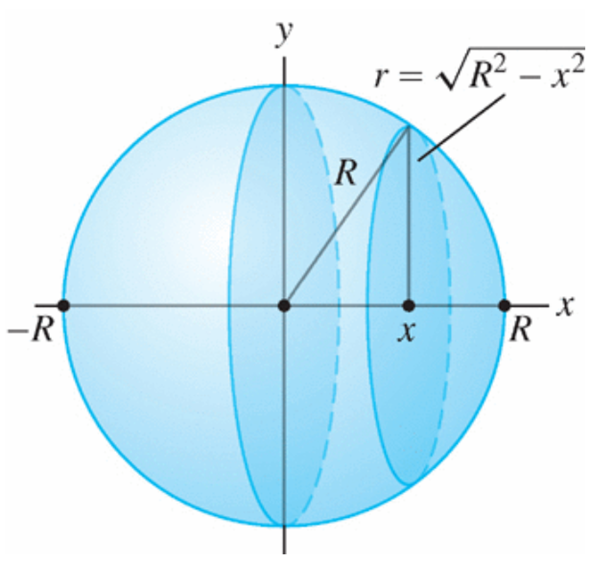
\includegraphics[width=.9\textwidth]{volumes/pictures/v2}}
\end{columns}

\uncover<4->{ Therefore, the sphere has volume}     
\[
\uncover<4->{\int_{-R}^R  \pi(R^2 - x^2)}\uncover<5->{= \pi\cdot \left.\left(R^2x-\frac{x^3}{3}\right)\right|_{-R}^R=2(\pi R^3-\pi\frac{R^3}{3})} \uncover<6->{= \frac43\pi R^3.}
\]
 %{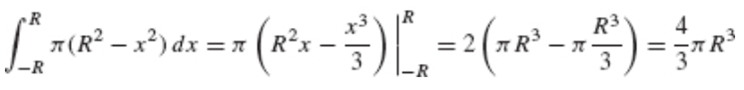
\includegraphics[width=\textwidth]{volumes/pictures/v3}}
\end{example}
\end{frame}


\begin{frame}\frametitle{Solid of revolution }
The Cross-section of a solid of revolution (about the x-axis) is a circle of radius $ f(x) $, and area $ \pi \left(f(x)\right)^2. $
{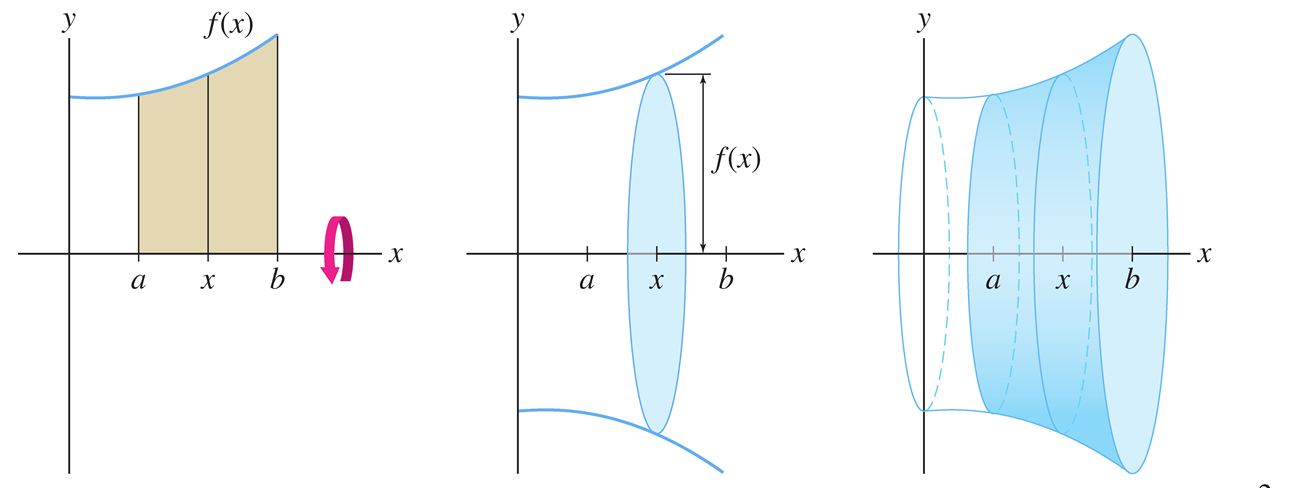
\includegraphics[width=.9\textwidth]{volumes/pictures/solid1}}
\end{frame}